%% This is file `elsarticle-template-1-num.tex',
%%
%% Copyright 2009 Elsevier Ltd
%%
%% This file is part of the 'Elsarticle Bundle'.
%% ---------------------------------------------
%%
%% It may be distributed under the conditions of the LaTeX Project Public
%% License, either version 1.2 of this license or (at your option) any
%% later version.  The latest version of this license is in
%%    http://www.latex-project.org/lppl.txt
%% and version 1.2 or later is part of all distributions of LaTeX
%% version 1999/12/01 or later.
%%
%% Template article for Elsevier's document class `elsarticle'
%% with numbered style bibliographic references
%%
%% $Id: elsarticle-template-1-num.tex 149 2009-10-08 05:01:15Z rishi $
%% $URL: http://lenova.river-valley.com/svn/elsbst/trunk/elsarticle-template-1-num.tex $
%%
\documentclass[preprint,12pt]{elsarticle}

%% Use the option review to obtain double line spacing
%% \documentclass[preprint,review,12pt]{elsarticle}

%% Use the options 1p,twocolumn; 3p; 3p,twocolumn; 5p; or 5p,twocolumn
%% for a journal layout:
%% \documentclass[final,1p,times]{elsarticle}
%% \documentclass[final,1p,times,twocolumn]{elsarticle}
%% \documentclass[final,3p,times]{elsarticle}
%% \documentclass[final,3p,times,twocolumn]{elsarticle}
%% \documentclass[final,5p,times]{elsarticle}
%% \documentclass[final,5p,times,twocolumn]{elsarticle}

%% The graphicx package provides the includegraphics command.
\usepackage{graphicx}
%% The amssymb package provides various useful mathematical symbols
\usepackage{amssymb}
%% The amsthm package provides extended theorem environments
%% \usepackage{amsthm}

%% The lineno packages adds line numbers. Start line numbering with
%% \begin{linenumbers}, end it with \end{linenumbers}. Or switch it on
%% for the whole article with \linenumbers after \end{frontmatter}.
\usepackage{lineno}

%% natbib.sty is loaded by default. However, natbib options can be
%% provided with \biboptions{...} command. Following options are
%% valid:

%%   round  -  round parentheses are used (default)
%%   square -  square brackets are used   [option]
%%   curly  -  curly braces are used      {option}
%%   angle  -  angle brackets are used    <option>
%%   semicolon  -  multiple citations separated by semi-colon
%%   colon  - same as semicolon, an earlier confusion
%%   comma  -  separated by comma
%%   numbers-  selects numerical citations
%%   super  -  numerical citations as superscripts
%%   sort   -  sorts multiple citations according to order in ref. list
%%   sort&compress   -  like sort, but also compresses numerical citations
%%   compress - compresses without sorting
%%
%% \biboptions{comma,round}

% \biboptions{}

\journal{Energy Policy}

\begin{document}

\begin{frontmatter}

%% Title, authors and addresses

\title{Study of Electricity Theft Impact on the Economy of a Regulated Electricity Company}


%% use optional labels to link authors explicitly to addresses:
%% \author[label1,label2]{}
%% \address[label1]{}
%% \address[label2]{}


\author[rvt]{L.G.~Arango\corref{cor1}\fnref{fn1}}
\ead{lucasarango10@yahoo.com.br}
\author[rvt]{E.~Deccache\fnref{fn1}}
\ead{elciodeccache@unifei.edu.br }
\author[rvt]{B.D.~Bonatto\fnref{fn1}}
\ead{bonatto@unifei.edu.br }
\author[rvt]{H.~Arango\fnref{fn1}}
\ead{hector.arango@uol.com.br }
\author[rvt]{E.O.~Pamplona\fnref{fn2}}
\ead{pamplona@unifei.edu.br}
%%\author[els]{E.O.~Pamplona\corref{cor2}\fnref{fn1,fn3}}
%%\ead[url]{pamplona@unifei.edu.br}
\cortext[cor1]{Corresponding author}
\cortext[cor2]{Principal corresponding author}
\fntext[fn1]{CERIn - Center of Excellence in Smart Grids}
\fntext[fn2]{IEPG - Management \& Production Engineering Institute \\Unifei - Federal University of Itajuba}

\address[rvt]{Unifei - Federal University of Itajuba \\ Av. BPS, 1303, Bairro Pinheirinho, Itajuba - MG}

\tnotetext[t1]{The authors would like to thank ELETROBRAS, ANEEL, INERGE, CAPES, CNPq and FAPEMIG for financially supporting this research.}

%% use the tnoteref command within \title for footnotes;
%% use the tnotetext command for the associated footnote;
%% use the fnref command within \author or \address for footnotes;
%% use the fntext command for the associated footnote;
%% use the corref command within \author for corresponding author footnotes;
%% use the cortext command for the associated footnote;
%% use the ead command for the email address,
%% and the form \ead[url] for the home page:
%%
%% \title{Title\tnoteref{label1}}
%% \tnotetext[label1]{}
%% \author{Name\corref{cor1}\fnref{label2}}
%% \ead{email address}
%% \ead[url]{home page}
%% \fntext[label2]{}
%% \cortext[cor1]{}
%% \address{Address\fnref{label3}}
%% \fntext[label3]{}


%% use optional labels to link authors explicitly to addresses:
%% \author[label1,label2]{<author name>}
%% \address[label1]{<address>}
%% \address[label2]{<address>}

\begin{abstract}
%% Text of abstract
The Electricity theft is an economic issue for the electricity company due to unbilled revenue of consumers who commit such action. In a regulated scenario the company needs to fit within the laws of a regulatory agency (ANEEL in Brazil) and the loss of revenue is a problem that can compromise the compliance with regulatory targets and business efficiency. The objective of this article is to analyze how the energy theft impacts on the economy of the regulated company, consumers and society as a whole. Through the economic model Tarot (Optimized Tariff) it was possible through a concise and comprehensive manner to analyze the regulated electricity market using simulations and discover in which points the company operates optimally and through it to determine the economic indicators.
\end{abstract}

\begin{keyword}
Electricity theft \sep Regulated Electricity Company \sep Economic Impact \sep Tarot \sep Operational Optimal Point.
%% keywords here, in the form: keyword \sep keyword

%% MSC codes here, in the form: \MSC code \sep code
%% or \MSC[2008] code \sep code (2000 is the default)

\end{keyword}

\end{frontmatter}

%%
%% Start line numbering here if you want
%%
\linenumbers

%% main text
\section{Introduction}
\label{S:1}

The sale of electricity is the main form of revenue for a power distribution utility. However, not all purchased energy from generators is sold to energy consumers. Part of the purchased energy is lost due to the electrical losses from the conditions and characteristics of the network and another part is lost in form of technical and commercial losses. The sum of technical losses with non-technical losses represents the global system losses. Non-technical losses on distribution represent a major impact on company revenue because of the energy that is not billed.\\
When the amounts of these losses begin to get too high the electricity utility should worry because its billed revenue become lower. An economic analysis will be done in this paper in order to demonstrate how these losses growth exclusively from electricity theft impact on the financial diagram of the company.
Moreover, an analysis of how the electricity theft affects the social indicators such as the consumer surplus and the social welfare will be carried out. \\
A study of the company in the regulated scenario with and without electricity theft will also be conducted in order to determine one or more optimized tariffs in order to obtain the economic added value of the electric utility equal to zero, which is a regulatory requirement imposed by ANEEL (the Brazilian electrical energy regulatory agency).\\
Other non-technical losses such as fraud, billing errors and measurement, among others, will not be considered in this article, which initially focuses exclusively on electricity theft \citet{Penin2008CombatPortuguese} \citet{Smith2004ElectricityAnalysis} \citet{Amin2015Game-theoreticInfrastructure}.\\
For countries in which electricity theft is not a problem, the economic model of this paper has also its importance. Thinking that electricity theft causes an unbilled revenue to the company, for other not billed revenues it can also be used as for example in frauds, government facilities which does not pay for electricity and so on.\\
Figure \ref{Fig1} represents the global energy losses on a subsystem segregated into technical and commercial losses and their subdivisions:\\

\begin{figure}[h]
\centering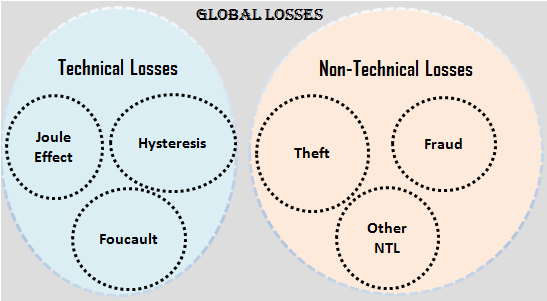
\includegraphics[width=0.8\linewidth]{Fig1.png}
\caption{Losses Representation of a Power System}
\label{Fig1}
\end{figure}


The electricity theft represents the deviated energy, or the energy that is not registered by the meter. Figure \ref{Fig2} illustrates this phenomenon:\\
The energy that leaves the transformer is lost in form of electrical losses and the energy that feeds the consumers is called required energy.\\
Where:\\

\begin{figure}[h]
\centering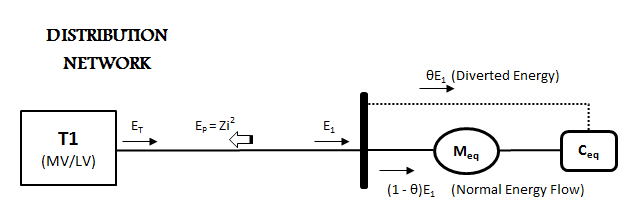
\includegraphics[width=0.8\linewidth]{Fig2.png}
\caption{Energy Theft Schematic in Distribution Network}
\label{Fig2}
\end{figure}

T1: Transformer.\\
M: Electrical Energy Meter.\\
$E_1$: Total energy supplied to consumers after technical losses.\\
$Ceq$: Equivalent Energy Consumer.\\

\section{Theoretical Reference}
\label{S:2}

\subsection{Consumer Model}
\label{SS:2-1}

A consumer model in general can be expressed by the amount of energy required in relation to the price of the electricity and its utility or value of use. If the utility, converted into monetary values provide a greater benefit than the payoff or the cost that the consumer will have to purchase the good, then it can be said that consumers are having an economic surplus, also known as consumer surplus. Figure \ref{Fig3} and equation \ref{eqA} can represent this statement:

%inserir figura 3
\begin{figure}[h]%btp]
\centering
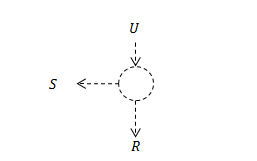
\includegraphics[scale=1]{Fig3.png} 
\caption{Consumers TAROT Model.}
\label{Fig3}
\end{figure}

\begin{equation}
\label{eqA}
S = U - R
\end{equation}

Where:\\

U: Consumers Utility in the use of Electricity.\\
R: Consumers Payoff / Electric Utility Revenue.\\
S: Consumers Surplus.\\

The electricity consumers can be represented by a linear model of consumption. The parameters that characterize consumer preferences by the product electricity can be synthesized through their eagerness and satiety. The curve that illustrates this model can be represented by the equation \ref{eqB}:\\
\begin{equation}
T = a - b*E
\label{eqB}
\end{equation}

Similarly the amount of consumed energy can be calculated by equation \ref{eqC}:\\
\begin{equation}
E = \frac{a-T}{b}
\label{eqC}
\end{equation}

So, consumer utility in acquiring the good energy is represented by the integral of the consumption curve in relation to energy as indicated in equation \ref{eqD}:\\
\begin{equation}
U=\int(a-b*E)dE= a*E-\frac{b*E^2}{2}
\label{eqD}
\end{equation}
Moreover,it is possible to calculate the energy purchased by the consumer, which can be expressed in the form of revenue for the electricity utility by equation \ref{eqE}:\\
\begin{equation}
R= T*E = (a-b*E)E = a*E - b*E^2
\label{eqE}
\end{equation}
Consumer surplus represents the difference between the utility and the revenue and it is represented by equation \ref{eqF}:\\
 \begin{equation}
S = U-R = \frac{b*E^2}{2}
 \label{eqF}
 \end{equation}
 
Where:\\

$a$: represents consumers eagerness.\\
$b$: represents consumers satiety.\\
$E$: represents the amount of energy available to purchase.\\
$T$: represents the energy Tariff.\\ 

\subsection{Electricity Utility Economic Model}
\label{SS:2-2}

The model of the electricity company in a regulated scenario can be represented by TAROT (Optimized Tariff economic model) presented on Figure \ref{Fig4}. \\
TAROT \citet{Arango2010TheMarkets}, \citet{Arango2008AValue}, \citet{Arango2008OOtima}, expresses the interaction of the electricity company with consumers who buys energy. Both providers and users are portrayed by sub-models whose objective is to combine simplicity with adherence to the actual conduct of market players.\\
The Appendix contains a brief description of both sub-models and how to combine them  to explain the electricity market model.\\
%Inserir a figura 4
\begin{figure}[h]%btp]
\centering
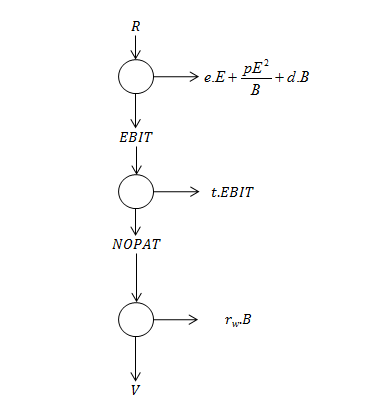
\includegraphics[width = 0.45\textwidth]{Fig4.png} 
\caption{Electricity Utility TAROT Model.}
\label{Fig4}
\end{figure}

Where:\\\\
%%$C= e*E+ \dfrac{p*E^2}{B} + d*B $ - costs of supplying energy where:\\
%%\begin{itemize}
$e*E$: Variable Costs.\\
$\frac{p*E^2}{B}$: are costs related to technical losses. \\
$d*B$: net depreciation or portion of investment.\\
$p, e, d$: are adjustable coefficients intended to approximate the costs to real situations.\\
B: Investment in physical system or network.\\
E: Energy sold.\\
%%\end{itemize}
EBIT: Earnings Before Interests and Taxes.\\
%t*EBIT – Taxes; Where
t: tax aliquot over EBIT.\\
NOPAT: Net Operating Profit After Taxes.\\
%Y =  – Capital Remuneration or WACC, where:\\
%\begin{itemize}
$r_w$: coefficient of return on capital invested.\\
B: Remuneration Basis or Investment.\\
V: Economic Value Added.\\
W: Economic Welfare Added.\\\\
%\end{itemize}
In the TAROT model of Fig. \ref{Fig4}, V can be expressed by equation \ref{eqG}:\\
\begin{equation}
V = (1-t)*\left( T*E - \frac{p*E^2}{B} - d*B - e*E \right)   - r_w *B
\label{eqG}
\end{equation}
And The Revenue by equation \ref{eqH}:\\
\begin{equation}
R = \frac{T}{b} * (a-T)
\label{eqH}
\end{equation}\\
The calculation of the optimal tariff is necessary in order to determine the value of the tariff that should be charged to electricity consumers in a regulatory situation. In other words, the situation where the economic added value of the electric company is equal to zero, which is a regulatory requirement of ANEEL.\\
Inserting equation \ref{eqC} into \ref{eqG} and assuming V=0, results in equation \ref{eqI}:\\
\begin{equation}
\alpha * T^2 +\beta * T + \delta = 0
\label{eqI}
\end{equation}\\

Where $ \alpha$, $\beta$ e $\delta $ are given by equations \ref{eqJ}-\ref{eqL}:\\
\begin{equation}
\alpha = -\frac{1}{b} - \frac{p}{b^2*B}
\label{eqJ}
\end{equation}

\begin{equation}
\beta = \frac{(a+e)}{b} + \frac{2*a*p}{b^2*B}
\label{eqK}
\end{equation}
\begin{equation}
\delta = -\frac{r_w *B}{1-t}- \frac{p*a^2}{b^2*B}-d*B- \frac{e*a}{b}
\label{eqL}
\end{equation}\\
Therefore, by using equation \ref{eqI}, it is possible to verify that there are two optimal values for the tariff (T) that lead the electricity company economic added value become zero, thus attending the regulatory paradigm. \\
These optimal tariffs points that meet the regulatory model are given by equations \ref{eqM} and \ref{eqN}:\\
\begin{equation}
T_1 = \frac{-\beta - \sqrt{\beta ^2 - 4* \alpha *\delta}}{2*\alpha}
\label{eqM}
\end{equation}
and:
\begin{equation}
T_2 = \frac{-\beta + \sqrt{\beta ^2 - 4* \alpha *\delta}}{2*\alpha}
\label{eqN}
\end{equation}\\

\subsection{Inserting Energy Theft in the Economic Model of a Regulated Company}
\label{SS:2-3}

As \citet{Arango2016ImpactQuality}, when there is the presence of electricity theft, it is observed an increase in the energy consumption of a subsystem. Thus, equations \ref{eqO}-\ref{eqQ} that express this increase can be represented as follows :\\
\begin{equation}
E_0 = E_F = \frac{a-T}{b}
\label{eqO}
\end{equation}
\begin{equation}
E_1 = (1-\theta)* \frac{1-T}{b}+\theta* \frac{a}{b} = \frac{a - T*(1-\theta)}{b}
\label{eqP}
\end{equation}
\begin{equation}
\Delta E_\% = \frac{\theta*T}{a-T} * 100
\label{eqQ}
\end{equation}\\
Where:\\\\
$E_0$: represents the amount of Energy in a situation with absence of Electricity Theft.\\
$E_1$: represents the amount of Energy in a situation with Electricity Theft.\\
$E_{1F}$: represents the billed Energy in a situation with Electricity Theft.\\
$\theta$: Percentage of Total stolen Energy.\\

The representation in the case of energy theft is a little different. The energy required for this case increases, which causes an increase in the variable costs of the company and also an increase in the costs of the system's technical losses. \\
In contrast, the power utility revenue decreases due to the reason that the energy thieves are not paying for it. In other words, the energy billed decreases. 
Figure \ref{Fig5} shows in diagrammatic form the economic analysis of the electric company for electricity theft case:

%Introduzir a figura 5
\begin{figure}[h]%btp]
\centering
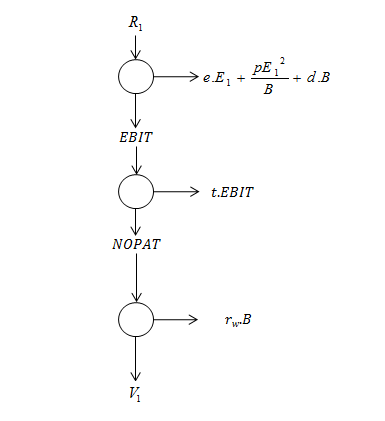
\includegraphics[width = 0.45\textwidth]{Fig5.png} 
\caption{TAROT Model of Electric Company with Energy Theft.}
\label{Fig5}
\end{figure}
In the electricity theft condition the revenues billed by the the company decreases with the amount of theft according to equation\ref{eqR}:\\
\begin{equation}
R_1 = T*(1-\theta)* \frac{a-T}{b}
\label{eqR}
\end{equation}\\
It is possible to verify that the share of energy billed by the electric company drops as the percentage energy theft  increases.\\
Moreover, the technical losses and operating costs for the electricity theft situation increase in relation to the case of theft absence. This can be easily explained because there is an increase in power consumption from the electricity theft given by equation \ref{eqQ}. \\
So, the economic added value of a company in a theft situation can be represented by equation \ref{eqS}:
\begin{equation}
V_1 = (1-T)*\left( T*E_{1F} - \frac{p*E^2}{B} - d*B -e*E_1\right) - r_w * B
\label{eqS}
\end{equation}\\

The calculation of the optimal tariff will occur in order to verify which tariff should be charged to electricity consumers in a regulatory situation. In other words, the situation where the electric company added value is equal to zero, which is a regulatory requirement of ANEEL.\\
After some algebraic developments it is possible to reach the equation \ref{eqT}:
\begin{equation}
\alpha_1 *T^2 +\beta_1 * T + \delta_1 = 0
\label{eqT}
\end{equation}
Where the parameters $\alpha_1$, $\beta_1$ e $\delta_1$ are calculated by the equations \ref{eqZ}-\ref{eqAB}:
\begin{equation}
\alpha_1 = \frac{\theta - 1}{b} - \frac{p*(1-\theta)^2}{b^2*B}
\label{eqZ}
\end{equation}

\begin{equation}
\beta_1 = \frac{(a+e)*(1-\theta)}{b}+\frac{2*a*p*(1-\theta)}{b^2*B}
\label{eqAA}
\end{equation}

\begin{equation}
\delta_1 = -\frac{r_w *B}{1-t}- \frac{p*a^2}{b^2*B}-d*B- \frac{e*a}{b}
\label{eqAB}
\end{equation}\\
That is, using the equation \ref{eqT}, it is possible to establish that there are two optimal points of tariff on a electricity theft situation that causes to an electric company the economic added value to be zero, respecting the regulatory paradigm.
Therefore:\\
\begin{equation}
T_1^* =  \frac{-\beta_1 -\sqrt{\beta_1^2 - 4*\alpha_1*\delta_1}}{2*\alpha_1}
\label{eqAC}
\end{equation}
\begin{equation}
T_2^* =  \frac{-\beta_1 +\sqrt{\beta_1^2 - 4*\alpha_1*\delta_1}}{2*\alpha_1}
\label{eqAD}
\end{equation}\\

Algebraically, through the proposed model it is possible to determine the threshold of electricity theft percentage in obtaining the optimal tariff. For this, the equation \ref{eqAE} must be obeyed:\\ 

\begin{equation}
\sqrt{\beta_1^2 - 4*\alpha_1*\delta_1}=0
\label{eqAE}
\end{equation}\\

Inserting equations \ref{eqZ}-\ref{eqAB} in equation \ref{eqAE} and solving it is possible to reach the equation \ref{eqU}:\\
\begin{equation}
\rho*(1-\theta)^2+ \omega*(1-\theta) = 0
\label{eqU}
\end{equation}\\

Where:\\
\begin{equation}
\rho= \frac{(a+e)^2}{b^2}+\frac{4*a^2 * p^2}{b^4 B^2} + \frac{4*a*p*(a+e)}{b^3 * B}+ \frac{4*\delta*p}{b^2*B}
\label{eqV}
\end{equation}

\begin{equation}
\omega = \frac{4*\delta}{b}
\label{eqX}
\end{equation}\\
Solving, it is possible to reach the energy theft threshold by the equation \ref{eqY}:

\begin{equation}
\theta_1 = 1 + \frac{4* \delta}{b * \rho}
\label{eqY}
\end{equation}\\

\begin{equation}
\theta_2 = 1
\end{equation}\\

That is, for values of $\theta$ greater than $\theta_1$, the electricity company can not get an optimal tariff to be able to balance its revenue with its costs. This can be explained by the fact that with the increase in electricity theft the company reduces its invoiced revenue. In contrast, their costs tend to increase due to the increase in energy consumption of the system. Thus, from a determined threshold value of energy theft, it becomes impossible for the electricity company to have its economic value added equal to zero.\\
Therefore, with company and consumer parameters it is possible to calculate the electricity theft percent threshold for any power distribution utility, which is a very valuable information in terms of how much the company must invest to reduce their theft in order to reach the region of the threshold value.\\

\section{Simulations without Electricity Theft}
\label{S:3}

In order to analyze how the theft of energy impacts on the economy of an electricity company, and more, consolidate and validate the proposed economic model, it is presented an analysis for a power distribution company without theft of energy and subsequently with electricity theft. \\
For this modeling, it will be used Tables \ref{tA} e \ref{tB}, that presents the consumer and company parameters for the economic market model:
The data from the Table \ref{tB} were extracted from \citet{ANEEL2008Second33/208.}.

\begin{table} [h]%btp]
\centering
\caption{Consumer Data}
%\begin{center}
\begin{tabular} {lll}
\hline 
\textbf{Symbol}&\textbf{Meaning}&\textbf{Value}\\
\hline
a&Eagerness&5300 [R\$/MWh]\\

b&Satiety&200 [R\$/$MWh^2$]\\
\hline 
\end{tabular}
%\end{center}
\label{tA}
\end{table}

\begin{table}[h]%btp]
\centering
\caption{Electric Utility Data}
\begin{tabular}{lll}
\hline
\textbf{Symbol}& \textbf{Meaning}& \textbf{Value}\\
\hline
T&Tariff&500 [R\$/MWh]\\
e&Variable Costs Coefficient&252 [R\$/MWh]\\
p&Technical Losses Coefficient&3600 [$(R\$/MWh)^2$]\\
B&Investment&3750 [MR\$]\\
d&Depreciation Coefficient&0,05\\
$r_w$&Investor Remuneration Percentage&7,26\%\\
t&Tax Rate on EBIT&34\%\\
\hline
\label{tB}
\end{tabular}
\end{table}

\subsection{Scenario without regulation}
\label{sec3-1}

Fig. \ref{Fig6} presents an analysis  of a scenario without regulation and in the absence of electricity theft, using data of Tables \ref{tA} and \ref{tB}:\\

%Inserir figura 6
\begin{figure}[h]%btp]
\centering
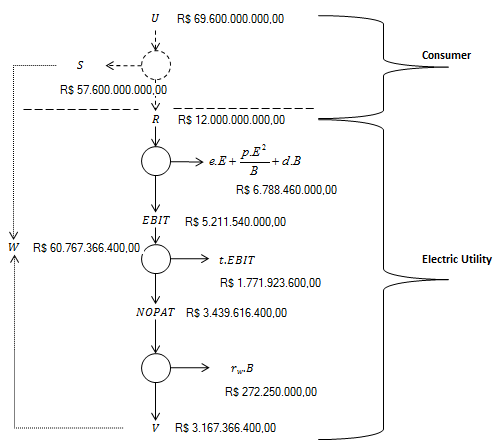
\includegraphics[width = 0.45\textwidth]{Fig6.png} 
\caption{Simulation of a non-optimal point with no Energy Theft.}
\label{Fig6}
\end{figure}

From Fig.\ref{Fig6}, it is possible to verify that the electricity company is having positive economic added value, which does not meet the regulatory requirements of ANEEL. Therefore, the company must choose an optimal tariff in order to have the added value equal to zero.\\

\subsection{Scenario with regulation}
\label{sec3-2}
Figure \ref{Fig7} represents the simulation with optimal tariff 1 and Figure \ref{Fig8} the simulation with optimal tariff 2:
%Inserir figura 7
\begin{figure}[h]%btp]
\centering
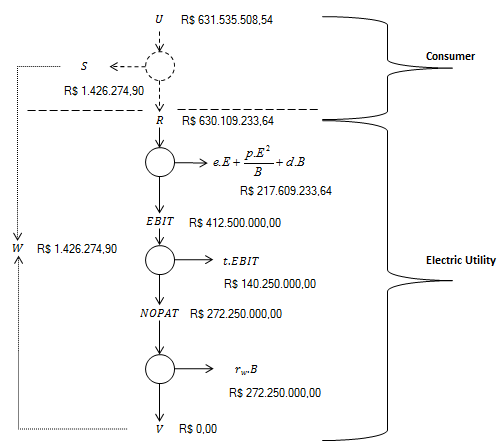
\includegraphics[width = 0.5\textwidth]{Fig7.png} 
\caption{Simulation at the point 1 of optimal tariff - Absence of Theft.}
\label{Fig7}
\end{figure}


%inserir figura 8
\begin{figure}[h]%btp]
\centering
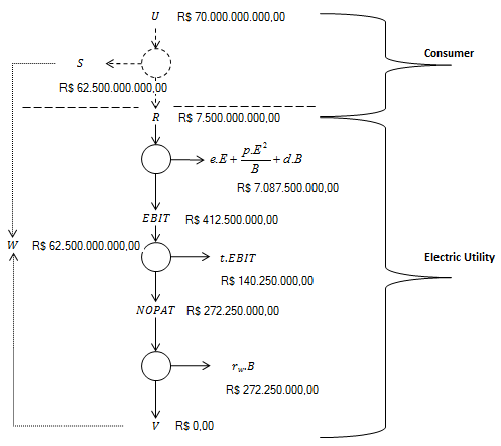
\includegraphics[width = 0.5\textwidth]{Fig8.png} 
\caption{Simulation at the point 2 of optimal tariff - Absence of Theft.}
\label{Fig8}
\end{figure}

\section{Simulations with Energy Theft ($\theta = 10$\%)}
\label{S.4}

In the following topics it will be developed simulations primarily based in an electrical company with a non-optimal tariff, representing an electricity utility in a deregulation situation. Subsequently, simulations will be performed with the utility's tariff at its optimum. As represented in the theoretical framework, the regulated company by the proposed model works in two points of optimum represented by $T_1^*$ e $T_2^*$.\\ 

\subsection{Electricity Utility working in a scenario without regulation}
\label{sec4-1}
Simulating with data on Tables \ref{tA} e \ref{tB} and inserting the electricity theft percentage of 10\%,   TAROT model presents the results for a not regulated electric utility shown by Figure \ref{Fig9} :\\

%Inserir figura 9
\begin{figure}[h]%btp]
\centering
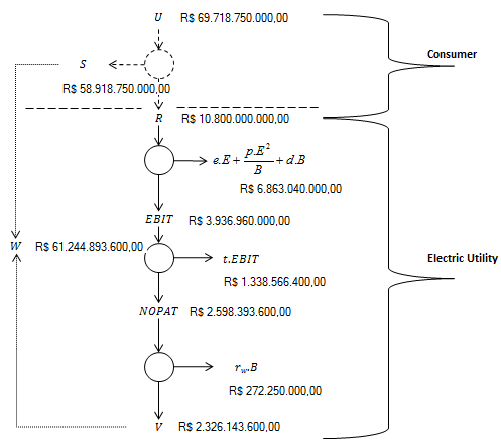
\includegraphics[width = 0.5\textwidth]{Fig9.png} 
\caption{Simulation of a non-optimal point with Energy Theft ($\theta$ = 10\%).}
\label{Fig9}
\end{figure}

Comparing with the same situation but with theft absence according to Figure \ref{Fig6}, it is possible to verify that the theft destroys economic value added to the electricity company. Moreover, the consumer surplus increase because of the increase on utility caused by the increase on consumption and decrease of the payoff in reason of some consumers not pay for electricity.

\subsection{Electric Utility working with optimized Tariff - Regulated Scenario}
\label{sec4-2}
The same simulation was done now, but with optimized tariffs ($T_1^* $ and $ T_2^*$). Figure \ref{Fig10} shows the case of optimal tariff 1 and Figure \ref{Fig11} shows the case of optimal tariff 2 :
%Inserir figura 10
\begin{figure}[h]%btp]
\centering
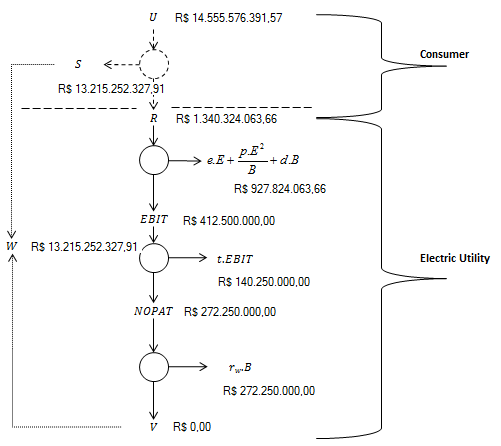
\includegraphics[width = 0.45\textwidth]{Fig10.png} 
\caption{Simulation on optimal tariff point 1 - Energy Theft ($\theta$ = 10\%).}
\label{Fig10}
\end{figure}

%Inserir figura 11
\begin{figure}[h]%btp]
\centering
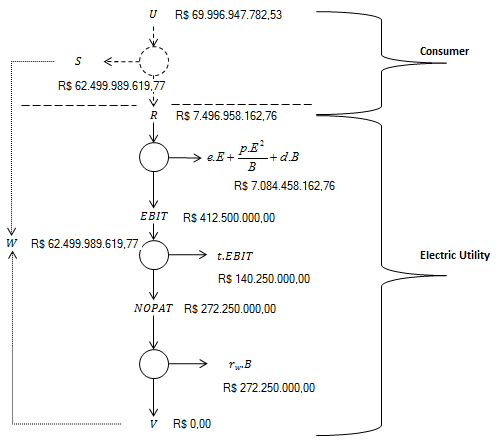
\includegraphics[width = 0.45\textwidth]{fig11.png} 
\caption{Simulation on optimal tariff point 2 - Energy Theft ($\theta$ = 10\%).}
\label{Fig11}
\end{figure}

\subsection{Threshold electricity theft percentage in achieving Optimized Tariff}
\label{sec4-3}
Using equation \ref{eqY} is possible to determine the threshold of the percentage of electricity theft to obtain the optimum tariff: \\
$\theta_1 = 0,79715$\\
That is, for energy theft value greater than 79,715 \%, it is not possible to obtain an optimal tariff, because that revenue is no longer able to cover the costs. \\

\subsection{Study of Theft Variation in the Economic Indicators of a Regulated Company (V=0)}
\label{sec4-4}
It is known, from the TAROT economic model, that a regulated company operates in two points of optimal tariff. \\
Through the generated simulations it was possible to assemble the following table with the main economic results of the electric company, consumers and government. \\
It is possible to verify by Tables \ref {tC} and \ref {tD} that for the company operating in the optimal point 1, the results of the consumer surplus and social welfare are worse than the company working at the optimum point 2. \\

\begin{table}[h]%btp]
\centering
\caption{Situation of optimal tariff 1 - (*All Values in [MR\$])}

\begin{tabular}{p{15mm}p{15mm}p{15mm}p{15mm}p{15mm}p{6mm}p{15mm}p{15mm}}%{llllllll}
\hline
$\theta $&$T_1^*$&U&R&S&V&W&G\\
\hline
0&5276,11&631,54&630,11&1,43&0&1,43&140,25\\
15\%&5223,35&20944,36&1701,55&19242,81&0&19242,81&140,25\\
30\%&5143,90&37811,87&2810,38&35001,49&0&35001,49&140,25\\
45\%&5012,78&51221,96&3959,34&47262,62&0&47262,62&140,25\\
60\%&4758,10&61169,19&5156,83&56012,36&0&56012,36&140,25\\
75\%&4012,64&67709,17&6457,12&61252,05&0&61252,05&140,25\\
79,71\%&2798,60&69419,39&7100,22&62319,17&0&62319,17&140,25\\
80\%&\multicolumn{7}{c}{It is not possible to obtain an optimal Tariff}\\

\hline
\end{tabular}

\label{tC}
\end{table}

\begin{table}[h]%btp]
\centering
\caption{Situation of Optimal Tariff 2 - (*All Values in [MR\$])}

\begin{tabular}{p{15mm}p{15mm}p{15mm}p{15mm}p{15mm}p{6mm}p{15mm}p{15mm}}%{llllllll}
\hline
$\theta$&$T_2^*$&U&R&S&V&W&G\\
\hline
0&300&70000&7500&62500&0&62500&140,2\\
15\%&356,8&69995,1&7495,1&62499,97&0&62499,97&140,2\\
30\%&440,2&69987,6&7487,8&62499,83&0&62499,83&140,2\\
45\%&575,3&69974,7&7475,3&62499,31&0&62499,31&140,2\\
60\%&834&69964,7&7449,6&62497,15&0&62497,15&140,2\\
75\%&1583,5&69833,2&7356,4&62476,80&0&62476,80&140,2\\
79,71\%&2798,6&69419,4&7100,2&62319,17&0&62319,17&140,2\\
80\%&\multicolumn{7}{c}{It is not possible to obtain an optimal Tariff}\\

\hline
\end{tabular}
\label{tD}
\end{table}
Moreover, increasing the percentage of electricity theft , the optimum tariff 1 starts to fall because the amount of energy increases. This occurs in reverse regarding to optimal tariff 2, in which the electricity theft leads the electric company to increase the tariff to balance their finances. \\

The payment for the government through taxes did not have a change because it is a percentage of EBIT. \\
It is possible to see that operating at the optimal tariff 1 and varying the percentage of theft, the company operates at higher tariffs and less energy. On the other hand, for the company operating at the optimal tariff 2, it achieves lower tariffs and higher amount of energy. \\
There is a threshold percentage of energy theft, wherein the electric company is not able to manipulate the tariff to obtain economic value added equal to zero. This fact can be explained because the billed revenue decline at a point that it would be unable to balance with their costs. Figure \ref{Fig12} illustrates this situation:\\


%Inserir figura 12
\begin{figure}[h]%btp]
\centering
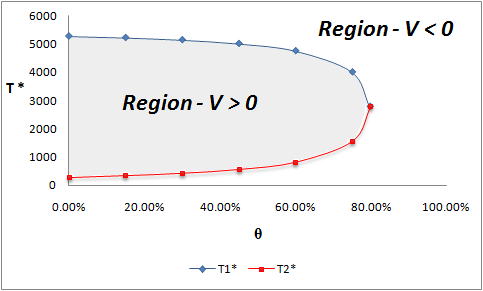
\includegraphics[width = 0.9\textwidth]{Fig12.png} 
\caption{Variation of the Optimized Tariff with Energy Theft of a Regulated Electric Company ($V = 0$)}
\label{Fig12}
\end{figure}
Therefore, the region inside the curves represents the set of points in which the company is adding economic value ($V > 0$). On the other hand, the region outside the curves represents the set of points in which the company is destroying economic value ($V < 0$).

\section{Conclusions}
\label{S.5}
Through the proposed economic market model it was possible to verify that a regulated electricity company can operate in two distinct points of optimal tariff. Looking to the consumer's perspective the higher optimal tariff causes a decrease in surplus, due to a higher payoff, reason by it becomes preferable the $T_2^*$.\\
The increase of energy theft in a regulated electric company (V = 0), caused a variation on optimized tariffs ($T_1^*$) e ($T_2^*$), leading to convergence as the theft reaches its threshold.\\
Through the parameters of the consumers and of the electricity utility, it is possible to determine the percent of theft threshold. That is, as consumers and utilities have different parameters, the theft threshold will be distinct. Therefore, it will not be appropriated if the regulator set the same theft goal to all electric utilities.\\
The electricity theft despite of reducing the economic value added of the company (V), increases the socioeconomic welfare (W). This can be explained by the fact that consumers are increasing their utility (consumed energy increase) and reducing its payoff (R), because they are not paying for energy. Thus, the consumer surplus (S) increases more than the reduction of the economic value added (V). Although the theft causes an increase in socioeconomic welfare (W), this act is considered illegal and regulators should in the first instance act in favour of what is ethically correct.\\

\section{Appendix}
\label{S.6}

TAROT (acronym for Optimized Tariff) is a model based on demonstration of the company's value. It combines the EVA calculation methodology, worldwide popularized by the company STERN and STEWART with $ANEEL$ regulatory procedure for tariff revision.
TAROT is based on a structure of expenditures (G), appropriate to electrical distribution system, which relates the costs in proportion to sales, technical losses and depreciation on investment.  Starting from the revenue (R), results taxable gains (EBIT = R - G) and taxes (X = t.EBIT).
Finally, capital remuneration is subtracted ($Y = r_w.B$) where (B) is the investment and ($r_w$) the cost of capital (WACC - Weighted Average Capital Cost).\\
%% The Appendices part is started with the command \appendix;
%% appendix sections are then done as normal sections
%% \appendix

%% \section{}
%% \label{}

\section{References}
\label{S.7}
%%
%% Following citation commands can be used in the body text:
%% Usage of \cite is as follows:
%%   \cite{key}          ==>>  [#]
%%   \cite[chap. 2]{key} ==>>  [#, chap. 2]
%%   \citet{key}         ==>>  Author [#]

%% References with bibTeX database:

\bibliographystyle{model1-num-names}
\bibliography{Mendeley_Tarot.bib}
%% Authors are advised to submit their bibtex database files. They are
%% requested to list a bibtex style file in the manuscript if they do
%% not want to use model1-num-names.bst.

%% References without bibTeX database:

% \begin{thebibliography}{00}

%% \bibitem must have the following form:
%%   \bibitem{key}...
%%

% \bibitem{}

% \end{thebibliography}


\end{document}

%%
%% End of file `elsarticle-template-1-num.tex'.